% Diese Datei ist jetzt UTF-8 codiert
% Bitte berücksichtigt das, wenn Umlaute einfügt!!!

\documentclass {beamer}

%\usepackage [ngerman] {babel}
\usepackage[utf8]{inputenc}
\usepackage[T1]{fontenc}
\usepackage{amsmath}
\usepackage{amssymb}

%\usepackage {beamerthemeshadow}
\usepackage{beamerthemeIlmenau}

\usepackage{alltt}
%\usetheme [compress] {Ilmenau}
%Ohne Navigation: default, boxes, Bergen, Bordilla, Madrid,AnnArbor, CambridgeUS, Pittsburgh, Rochester
%Mini Navigation: Berlin, Ilmenau, Dresden, Darmstadt, Frankfurt,Singapore, Szeged
%\usepackage {multimedia }
%\usepackage{epsfig}
\usepackage{graphicx}
%\usecolortheme {dove}
\usecolortheme{beaver} 
\beamertemplatenavigationsymbolsempty

 

\begin{document}

%\setbeamercolor{palette quaternary}{fg=white}  
%\usecolortheme {albatross, beetle, crane, dove, seagull, wolverine, beaver}
\title{Morphisto - \\ A Service-oriented Open Source Morphology for German}
\author{Andrea Zielinski, Christian Simon, Tilman Wittl}
\date{04.09.2009}

\frame{\titlepage}

\frame{
	\tableofcontents
	}

%\section{Morphisto - An Open Source Morphological Analyzer for German}

\section{Motivation}
\frame{
  \frametitle{Why did we need another Morphological Analyzer for German?}
\begin{itemize}
  \item{Morphisto originated within the context of the \textit{TextGrid} project, an infrastructure for e-Humanities}
  \item{Morphological analysis is the basis for a range of applications provided}
\begin{itemize}
  \item{Lemmatization}
  \item{Lexical Lookup in Dictionaries}
  \item{Annotation of Texts}
  %\item{Translation from/into other language stages of German}
\end{itemize}
  \item{No open-source morphological analyzer available for German at present}
  \item{except SMOR, but which lacks an open-source lexicon}
\end{itemize}
}

\subsection{Basic Idea}
\frame{
  \frametitle{Basic Idea}
\begin{itemize}
  \item{use GPL-licensed SMOR morphology for German (University of Stuttgart) as a starting point}
  \item{define lexical entries for the most common 30,000 German words as defined by the German 
reference word list (\textit{DeReWo})}
  \item{manage lexical data with the help of a relational database}
   %\item{Implement additional tools for the management of the lexical data}
  \item{partially aquire data from freely available sources (e.g. Adelung lexicon)}
  \item{integrate Morphisto as a series of easy-to-use web services for use in TextGrid infrastructure}
\end{itemize}
}

\subsection{Short Introduction to SMOR}
\frame
{
  \frametitle{SMOR}

SMOR is ...
  \begin{itemize}
  \item a computational morphology for German
  \item FST-based (SFST toolkit, cf. Schmid 2004)
  \item licensed under the GPL (except the lexicon)
  \end{itemize}
}

\frame
{
  \frametitle{What it can do}
SMOR analyzes inflectional forms of German
  \begin{itemize}
  \item<1->{simple (or compound) lexemes}
  \item<2->{derivational constructions}
  \item<3->{complex word formations need not be stored in the lexicon but can be analyzed on-the-fly}
  \item<4->{flat analyses:}
  \begin{alltt}
    Bahn<NN>Hof<NN>Halle<+NN><Fem><Nom><Sg>
  \end{alltt}
  \end{itemize}
}

\section{Bootstrapping a Morphological Analyzer}
%was zum Teufel ist ein MRD???
%\subsection{Extracting morphological information from a MRD}
\frame
{
  \frametitle{Lexical Aquisition for Morphisto}
Resources used:
\begin{itemize}
\item DeReWo Lemma List \url{http://www.ids-mannheim.de/kl/derewo/}
\item Adelung(1793) - Grammatisch-kritisches Wörterbuch der Hochdeutschen Mundart\newline 
\url{http://www.zeno.org/Adelung-1793}; lexicon published by the ``Digitale Bibliothek"; early NHD dictionary, free for the public, covering more than 65,000 entries
\item Deutsches Fremdwörterbuch (IDS Mannheim)
\item grammis (on-line grammar of the German language) \\
	\url{http://hypermedia.ids-mannheim.de/pls/public/gramwb.ansicht}
\end{itemize}
}

% bitte nicht Adelung....

%\frame{
%\frametitle{Example Entry from Adelung(1793)}
%An excerpt lemma entry from Adelung (1793) from which we aquired our data is given below:
%\begin{enumerate}
%\item Das Futter, des -s, plur. ut nom. sing. die Bekleidung eines Körpers von außen oder von innen; [..] 
%\item Das Futter, des -s, plur. ut nom. sing. 1) Alles, was Menschen und Thieren zur Nahrung dienet; ohne Plural [..] 
%\end{enumerate}
%}

%\subsection{Managing the Lexical Data}
\frame
{
  \frametitle{Managing the lexical data}
\begin{enumerate} 
\item in a relational database aquired data was outer-joined with DeReWo lemma list
\item the data was manually revised and completed with the goal that an automaton 
based mainly on German simplexes covers DeReWo lemma list
\item an XML-based exchange format was developed from which the data can be converted to the SFST automaton specification format
\end{enumerate}
}

%\frame
%{
%  \frametitle{Lexical Database Scheme }
%  What is needed?
%\begin{itemize}
% \item An exchange format that is independent of the specific finite-state platform
%\item Scripts that convert lexical data to the originial SMOR lexicon format
%\item Validating the lexicon against a schema
%\item Enhanced user interface for lexicographic work 
%\end{itemize}
%}


\frame
{ \frametitle{Conversion of an XML-based Lexical Entry to SMOR}

\begin{figure}
\begin{alltt}
<smor>\\
\hspace{1cm}<BaseStem>\\
\hspace{2cm}<Lemma>Atlas</Lemma>\\ 
\hspace{2cm}<Stem>Atlanten</Stem>\\
\hspace{2cm}<Pos>NN</Pos>\\
\hspace{2cm}<Origin>nativ</Origin>\\
\hspace{2cm}<InfClass>NMasc/Pl</InfClass>\\
\hspace{2cm}<Frequency>676</Frequency>\\
\hspace{1cm}</BaseStem>\\
</smor>\\
$\Rightarrow$<Basestems>Atlas:n<>:t<>:e<>:n<NN><base><nativ><NMasc/Pl>
\end{alltt}  

\caption{Example Conversion for \emph{Atlas (atlas)} }
\end{figure}
}

%\subsection{Cycle of Testing an Reengineering}

\frame
{ \frametitle{Morphisto's Contribution to SMOR morphology}
\begin{itemize} 
%\item Checking the analysis of the DeReWo list (on the Adelung transducer)
\item Morphisto's lexicon encompasses ca. 18,000 entries (lexicon provided by SMOR ca. 1,000)
%\item Adding missing base stems (for about 5,000 entries)
\item false inflection classes or features were added/corrected (e.g., for \emph{Geister} (ghosts)) 
\item word formation rules were added (e.g., for \emph{StudentIn/Innen} (male and/or female student(s))
\item so were rules for the derivation of compound or derivation stems (e.g., \emph{Peters-kirche} (Peter's church))
\end{itemize}
}

%\frame
%{ \frametitle{Intermediate Result}
%\begin{itemize} 
%\item Manually creating the simplex units together with their required features is time-consuming
%\item In the worst case, an intensive study of the documentation and software code is required
%\item Gold standard would be beneficial %as only the delta of analysis that has been affected by %rebuilding the network needs to be reanalyzed.
%\item Fine-tuning for stems and affixes that were likely to produce ambiguities
%\begin{itemize}
%\item Include complex words that produce segmentation errors (e.g., \textit{Tee-nager} (tea rodent) %instead of \textit{Teen-ager})
%into the lexicon
%\item Assign the tag <NoDef> or <Initial> to short or antiquated words to restrict their productivity
%\end{itemize}
%\end{itemize}
%}

\section{Test Results and Discussion}

\begin{frame}
\frametitle{Transducer Lexicon Statistics for Adelung and Morphisto}
\begin{small}
\begin{table}[h] 
\begin{center}
\begin{tabular}{|l|c|c|}
\hline
\textbf{Lexicon} & \textbf{Adelung} & \textbf{Morphisto} \\
\hline
\hline
Basestems &	32152 &	17339 \\
\hline
-	Nouns 	& 20605 &	7833 \\
-	Proper Nouns &	2	& 1053 \\
-	Verb stems &	7426 &	4300 \\
-	Adjectives  &	4061	& 3178 \\
-	Adverbs 	& 2	& 781 \\
-	Closed Word Classes &	28 &	190 \\
\hline
Derivation Stems & 	63 & 	67 \\
\hline
Compound Stems	& 30	 & 181 \\
\hline
Prefix Stems	& 94	& 213 \\
\hline
Suffix Stems (Derivation Rules) & 	404 & 	410 \\
\hline
\end{tabular}
\caption{Frequency of morphological units in the transducer lexicons}
\end{center}
	  \end{table} 
\end{small}
\end{frame}

\frame
{
\frametitle{Evaluation on the 'Ispell Test Corpus'}
The wordform list provided by German Ispell has been used for the evaluation of Morphisto. 
Approximately 225.833 words 
% 248.578 words - 22.745 DeReWo words 
of Ispell are unknown to Morphisto. 
The tests on randomly selected subsets of 100 inflected German wordforms in the different frequency ranges reveal the number of correct, missing and spurious readings, e.g. the precision and recall rates.  
}

\frame
{
\frametitle{Evaluation on the 'Ispell Test Corpus'} 

\smallskip
\begin{table}[h] 
\begin{center}
	\begin{tabular}{ | p{3,2cm} |  p{1,6cm} | p{1,5cm} | p{2,0cm} |}
	\hline
\textbf{Frequency Classes} &  \textbf{Precision} & \textbf{Recall} & \textbf{F-Measure} \\
\hline
$F_{0} - F_{4}$ &  100.00 & 100.00 & 100.00 \\
\hline
$F_{5} - F_{8}$ &  99.63 & 99.63 & 99.63 \\
\hline
$F_{9} - F_{12}$ &  98.74 & 87.71 & 92.90 \\
\hline
$F_{13} - F_{16}$ & 98.25 & 93.85  & 95.39 \\
\hline
$F_{17}$ - $F_{20}$&  93.21 & 84.36 & 88.56 \\
\hline
$F_{21}$ - $F_{25}$  & 91.77 & 81.00 & 85.33 \\
\hline
\hline
Average &   96.93 & 91.09 & 93.63\\
\hline
\end{tabular}	
\caption{Test results on ispell for different frequency classes}
\end{center}
\end{table} 
\smallskip
}

\subsection{Discussion}

%\frame
%{\frametitle{FSTs in Computational Morphology}
%Plus
%\begin{itemize} 
%\item A declarative framework for describing models
%\item Phonological regularities are described by use of context dependent rewrite rules 
%\item Search efficiency is improved via optimization algorithms (minimization, determinization, epsilon removal)
%\item Integrate filtering constraints via composition operations
%\end{itemize} 
%Minus
%\begin{itemize} 
%\item Filter rules generate a huge network
%\item Search space increases, and huge memory is required
%\end{itemize}
%}

\frame
{  
\frametitle{Remaining Issues}
Of course, Morphisto is still far away from being perfect. \\
Some of the remaining issues are:  
\begin{itemize}
  \item<1-> Different Segmentations \\
   West-europa vs. Weste-ur-opa 
  \item<2-> Ambiguous Constituents \\
   der/die Chile-Kiefer 
  \item<3-> Different Levels of Decomposition \\
     F\"uller vs. F\"ull-er \\
  \item<4-> Only rudimentary support for unknown lexical stems ("guessing")
\end{itemize}
\uncover<5>{Morphisto produces about 5 analyses on average!\\
  But: Humans often conceive only one reading for seemingly ambiguous words}
}

% Tilman, ab hier musst Du ran!!

\section{Improving the Morphological Analyzer}

\frame
{  \frametitle{Dealing with Ambiguous Analysis}
Idee:\\
Define a Language Model (LM) that captures the likelihood of a morpheme sequence to filter out unlikely analyses \\
Motivation
 \begin{itemize}
\item Task is similar to PoS Tagging 
\item Hidden Markov Models (HMMs) are used a lot in unsupervised morphology learning
\item Rank all hypothesis according to the Language Model \\
in a postprocessing step
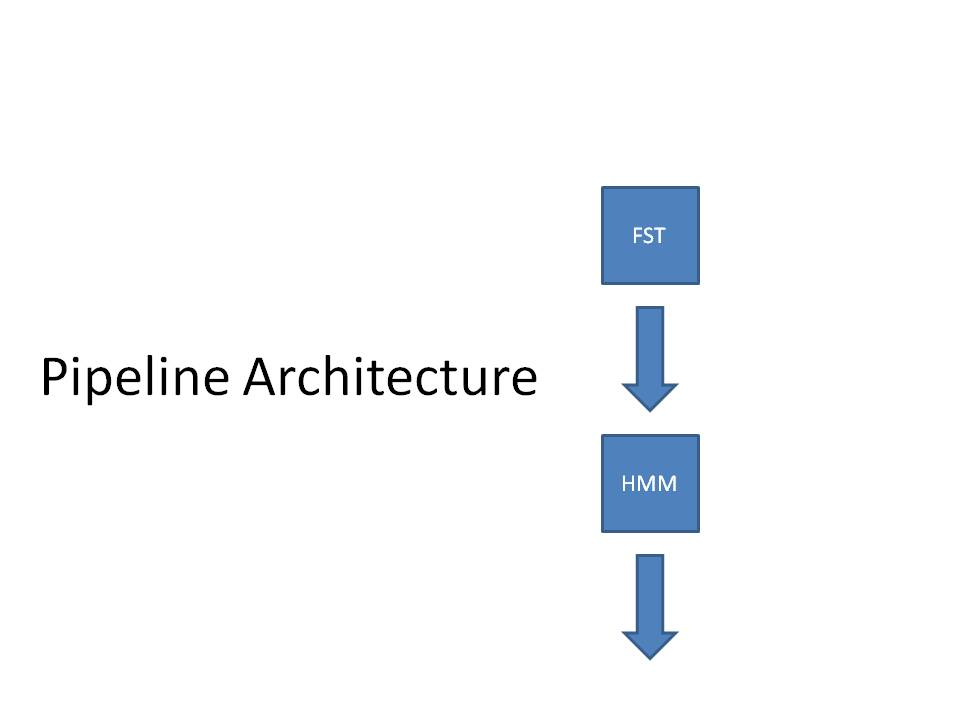
\includegraphics[width=5cm] {Pipeline2.jpg}
 %\item Adjust lexical probabilities from DeReWo frequency statistics 
\end{itemize}
}
%This way, the analysis with the fewest constituents is not automatically favoured. 
%Note: There are restrictions based on the part of speech for derivations. For example nominal case suffixes 
%can follow only nominal stems. These are already integrated declaratively.
%But In German we have a free compounding of morphemes. This is handled by the follwing rule:
 
 
 \frame
{  \frametitle{A Language Model for Morpheme Sequences}
%HMMs are a specific transducer models. In speech they are used to map states to phonemes
% P(W) = language model (likelihood of a morpheme sequence)
% P(Y|W) = acoustic model (likelihood of observed acoustic signal given word sequence)
- PoS tag of a morpheme depends on its context (conditional word class probabilities and lexical probabilities)\\
  \begin{itemize} 
  \item \textit{parken$<$V$>$Verbot$<$+NN$>$}  \\
  \item \textit{Park$<$NN$>$Verbot$<$+NN$>$}  \\
  \end{itemize}
- Learn different PoS tag sequences from a manually annotated corpus of correct analyses (10,000 words)\\
 \begin{itemize}
\item  bigram prob.: $<$V$>$<$N$>: 0.6, lexical prob. (park$|$V) = 0.55
\item  bigram prob.: $<$N$>$<$N$>: 0.4, lexical prob. (park$|$N) = 0.45
\end{itemize}
- Disambiguate morphemes in the context of the whole word\\
  \begin{itemize}
  \item Word with morphemes \begin{math} W = m_{1} ... m_{n} \end{math}
  \item Tag sequence \begin{math} T = t_{1} ... t_{n} \end{math}
    \end{itemize}
%estimate Language Model  
 }

\frame
{  \frametitle{Issues}
\begin{itemize} 
\item Training the Language Model
\item Finding the path with the highest likelihood in the integrated morphological network
\item Smoothing
\end{itemize}
For implementation details cf. Wittl, Tilman (2009): German Morphological Disambiguator based on statistical data. In: Proceedings of TaCoS 2009.
}

\frame
{  \frametitle{Future Work}

Transfomation into a Weighted Transducer (WFST) \\
e.g. HFST, a new open-source interface to existing transducer frameworks with many add-ons  \\
\begin{itemize} 
\item SMOR grammar should be reimplemented to profit from this
\item Problems: WFST will yield even more states
\item Which weight function? Probabilities, log probabilities, costs
\item Adjustement of weights by computing lexical probabilities from DeReWo and/or use of different measures (MI, C-Value, etc.) for word class probabilities
 \end{itemize}
 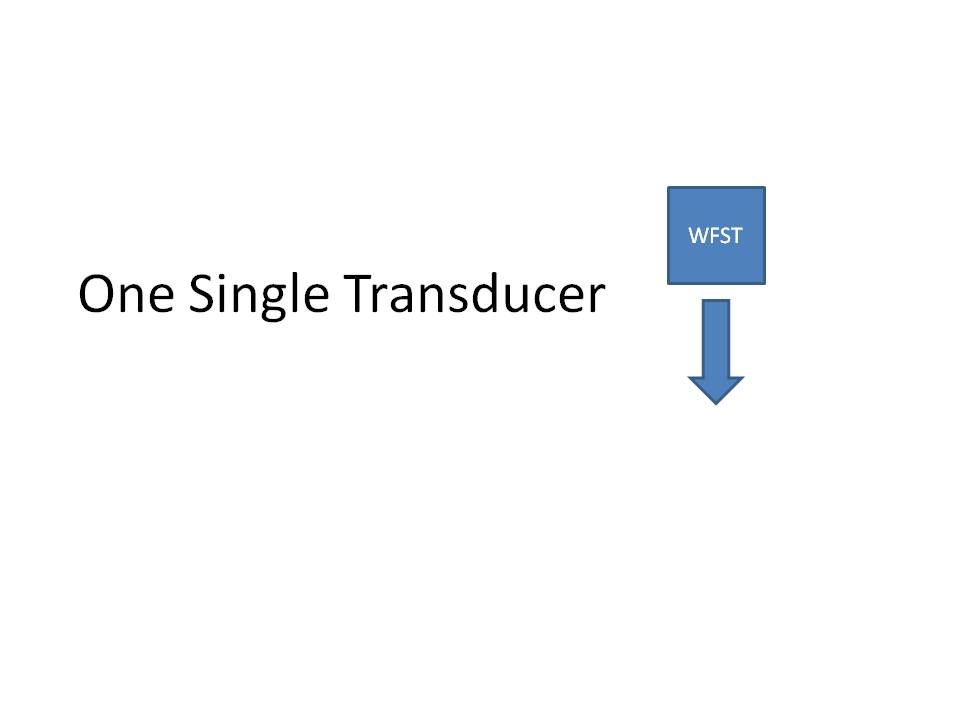
\includegraphics[width=5cm] {Single2.jpg}
}
%\begin{block}{Complete Morphological Model}
%LexModel = best path  D .o. LM \\
%where D is the dictionary transducer and LM is the language model, \\
%while .o. represents transducer composition.
%\end{block}
%One of the strengths of the WFST-based approach is the ease it provides for combining different knowledge
%sources (KSs). 
%New Operation: Search best path
%The main task for incorporating a new type of information into the overall Morphological Model is
%to convert it to WFST format %while the combination is carried out with the elegant composition algorithm

\frame
{  \frametitle{Graphics of a weighted transducer}
Example:
\begin{figure}[hp]
	\centering
		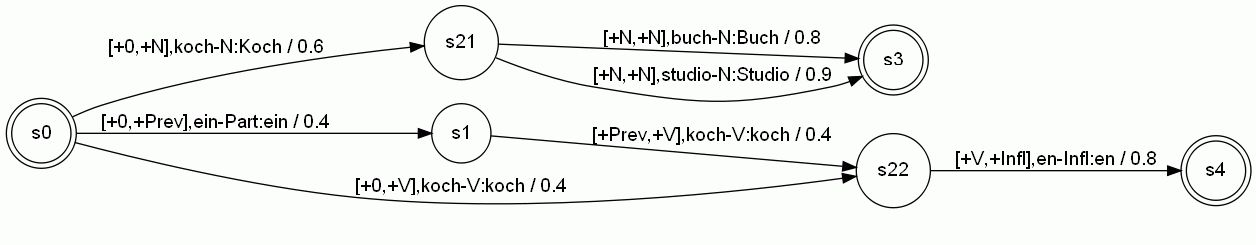
\includegraphics[width=10cm]{graph13.jpg}
	\label{fig:graph13}
\end{figure}
}

% Tilman, hier ist Dein Teil vorbei und ich übernehme wieder ....

\section{Morphisto in Real-World Applications}

%\subsection{Morphisto Analyzer/Generator at the IDS}
\frame
{  
	\frametitle{Online Demos of Morphisto}
%
\includegraphics[scale=0.75]{Workbench.jpg} 
 \begin{itemize}
 \item \htmladdnormallink{Morphisto at the IDS Mannheim:}{http://www.ids-mannheim.de/ll/TextGrid/morphisto.html}
\item  \htmladdnormallink{Wordform Analysis with Morphisto}{http://ingrid.daasi.de/cgi-bin/analyze.cgi}
\item  \htmladdnormallink{Generation of Inflection Table with Morphisto}{http://ingrid.sub.uni-goettingen.de/cgi-bin/flextables.cgi} 
\end{itemize}
You are welcome to download our Morphisto Transducer Lexicon for German 
}

% Baustelle:

\frame
{
  \frametitle{Morphisto in the elexiko Project}  
\begin{itemize}
 \item elexiko is freely available online dicionary of German
 \item based on lemma list encompassing 300,000 entries
 \item approx. 1,000 word articles have been finished so far
 \item Morphisto aims at providing automatically generated inflection tables 
 \item generation automaton created throgh SQL-based heuristics that reduce compounds to their heads
 \item elexiko lexicographer makes the final corrections which in turn are integrated into the Morphisto database
 %\item Example Entry in the field \textit{Wordformation} \\
 % \htmladdnormallink{elexiko-Stichwortliste}{http://www.owid.de}\\
\end{itemize}
 %\small {
 % \itshape{Antragsberatungskommission}\\
%	\begin{alltt}
%	\hspace{0,5cm}  Wortbildungsart/-typ:	Determinativkompositum, endozentrisch \\
%	\hspace{0,5cm}  Bestandteil: \textbf{Antrag}   Wortart: Nomen\\
%	\hspace{0,5cm}  Bestandteil: \textbf{Beratungskommission}   Wortart: Nomen\\
%	\hspace{0,5cm}  Fuge: -s- \\
%	\hspace{0,5cm}  Weitere Informationen unter canoo.net
%	\end{alltt}
%$\Longrightarrow$ Generate Information Automatically
}

%\subsection{Integration into TextGrid}
\frame
{  \frametitle{Servic-base Integration into TextGrid}
TextGrid distributes functionality over geographically distant grid servers.\\
Morphisto is integrated in TextGrid a set of web services providing functionality of
\begin{itemize} 
\item one-word morphological analysis and lemmatization
\item batch processing of utf-8 encoded word lists
\item annotating XML-based texts with lemma and morphological information
\end{itemize}
}

\frame
{
	\frametitle{Pros}
	Providing Morphisto's functionality via web-services offers independence from
	\begin{itemize}
	\item platform
	\item programming language \\
	(TextGrid's IDE is a Java-based RCP running on most major end-user systems)
	\item memory and cpu capacities on client machine
	\item installed SFST binaries on client system
	\end{itemize}
}

\frame
{
	\frametitle{Issues}
	\begin{itemize}
	\item<1-> size of automatons
		\begin{itemize}
			\item{DeReWo-based standard automaton alone has a size of 24 MB} 
			\item{all SFST compact automatons have a total size ca. 150 MB}
		\end{itemize}
	\item<1-> loading 24 MB into memory is extremely inefficient for processing one single wordform
	\item<2-> especially when considering that several queries must be processed at the same time (concurrency)
	\item<3-> certain input and configuration may require to run queried wordform through a different automaton if first automaton yielded no result (e.g. guessing)
	\end{itemize}
}

\frame
{
	\frametitle{Solution}
	\begin{itemize}
		\item<1-> \textit{fst-infl2} only used for processing large input files where no interaction is necessary
		\item<2-> for processing input files requiring "interaction" fst-infl2 was patched such that the Python web service can "chat" over the UNIX pipe 
		\item<3-> for processing small input (e.g. only a single wordform) a daemon was implemented that keeps all automatons in the memory of the server
	\end{itemize}
}

\frame
{
	\frametitle{Morphisto Daemon}
	\begin{itemize}
	\item<1-> the Daemon is memory-resistent unix tool running on the remote server that provides the web service
	\item<2-> implemented in Python using \textit{asynchat} module for asynchronous communication over a UNIX port
	\item<3-> loads Morphisto automatons only once at startup 
	\item<4-> runs queried wordforms through in-memory automatons
	\item<5-> uses TCP for flow control, which makes it more reliable, but also slower
	\end{itemize}
}

\frame
{  \frametitle{A Grid-based Demo}
%
\includegraphics[scale=0.5] {TextGrid.jpg}
%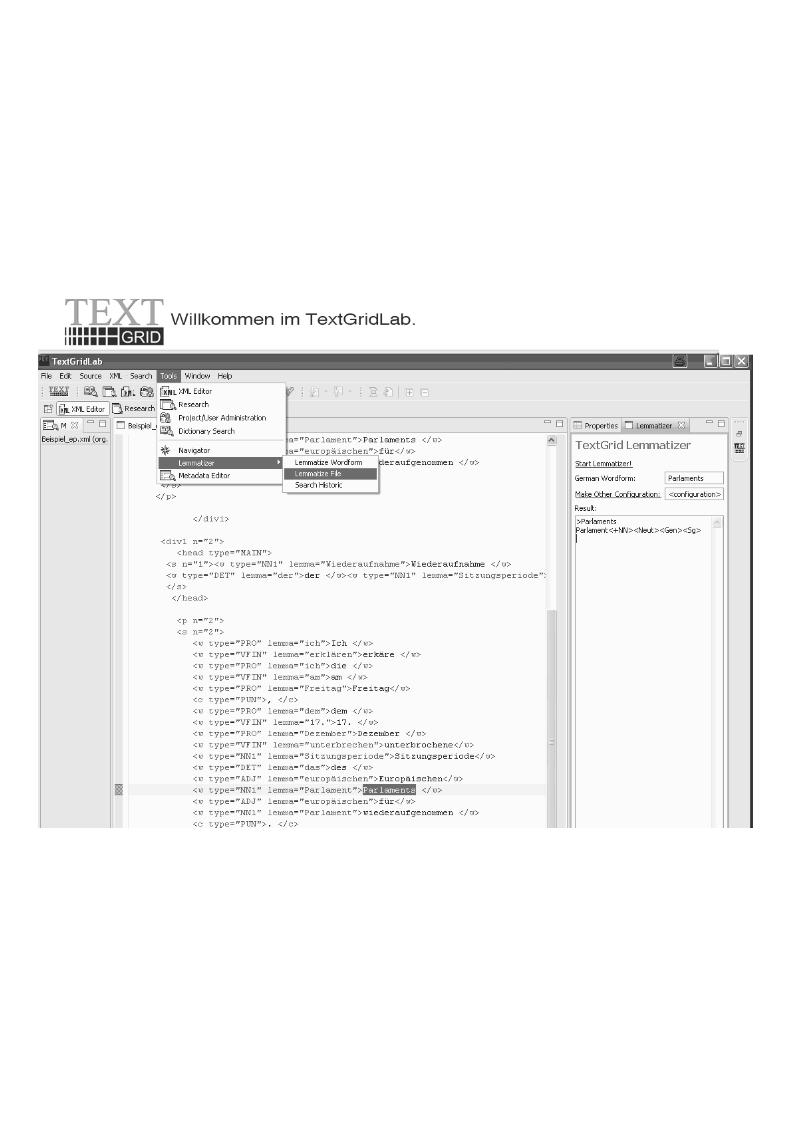
\includegraphics[width=7cm] {morpholymp1.jpg}
%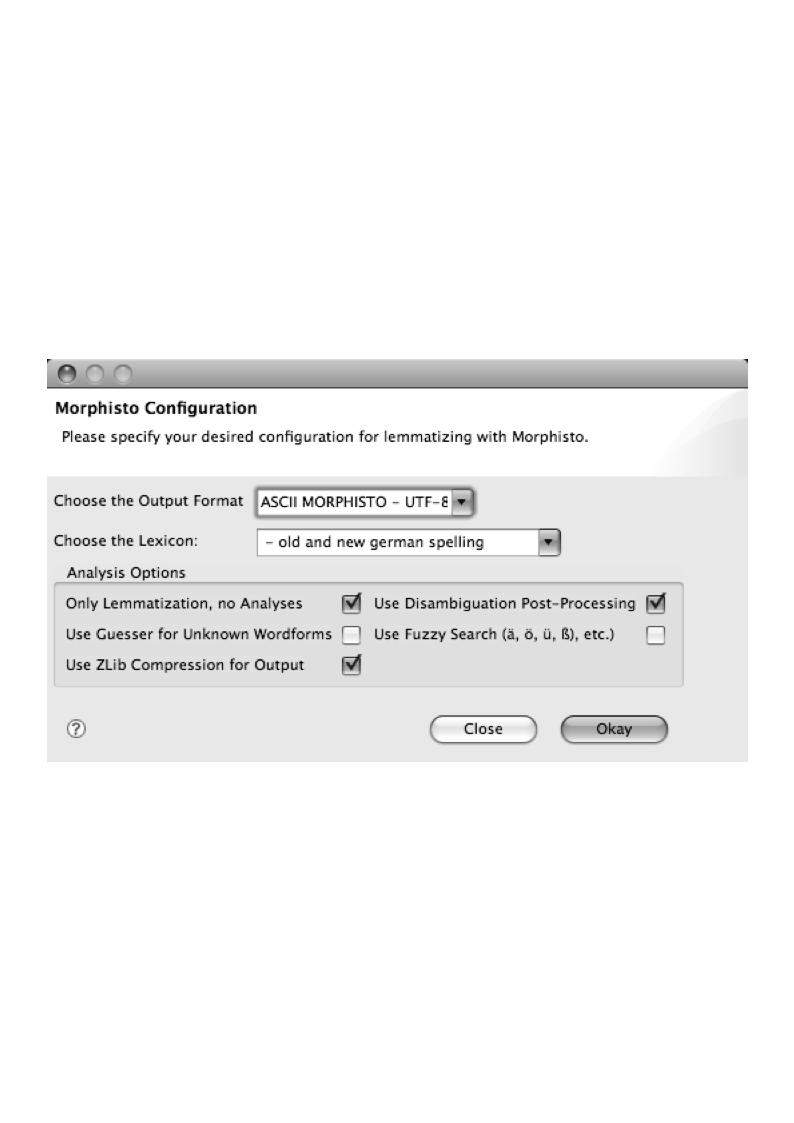
\includegraphics[width=7cm] {configuration3.jpg}
\begin{itemize}
\item{TextGrid Hompage \\ http://www.textgrid.de}
\item{elexiko Homepage \\ http://www.elexiko.de}
\item{Morphisto at Google Code \\ http://code.google.com/morphisto \\
Everybody is welcome to participate!}
\end{itemize}
}


\end{document}